% RUN pdflatex doc
% RUN biber doc
% RUN pdflatex doc
% PROFIT!

\documentclass[a4paper, 12pt]{article} % Font size (can be 10pt, 11pt or 12pt) and paper size (remove a4paper for US letter paper)

\usepackage{filecontents}

\usepackage[latin1]{inputenc}

\usepackage{biblatex}
\addbibresource{doc.bib}

\usepackage[protrusion=tr\"u,expansion=tr\"u]{microtype} % Better typography
\usepackage{graphicx} % Required for including pictures
\usepackage{wrapfig} % Allows in-line images

\usepackage{mathpazo} % Use the Palatino font
%\usepackage[T1]{fontenc} % Required for accented characters
\linespread{1.50} % Change line spacing here, Palatino benefits from a slight increase by default

%For lists/enumerations with small line distance: \begin{compactenum}
\usepackage{paralist}

\usepackage{minted} %Syntax highlighting
\usepackage{etoolbox} %Change minted line spacing
\AtBeginEnvironment{minted}{\singlespacing%
    \fontsize{10}{10}\selectfont}

\makeatletter
%\renewcommand\@biblabel[1]{\textbf{#1.}} % Change the square brackets for each bibliography item from '[1]' to '1.'
%\renewcommand{\@listI}{\itemsep=0pt} % Reduce the space between items in the itemize and enumerate environments and the bibliography

\renewcommand{\maketitle}{ 
\begin{flushright} % Right align
{\LARGE\@title} % Increase the font size of the title

\vspace{50pt} % Some vertical space between the title and author name

{\large\@author}
\\\@date 

\vspace{40pt}
\end{flushright}
}

\title{\textbf{Kademlia DHT}\\ % Title
Projektarbeit} % Subtitle

\author{\textsc{Moritz G\"ockel} % Author
\\{\textit{Hochschule Karlsruhe Technik und Wirtschaft}}} % Institution

\date{\today}

\begin{document}

\maketitle

\vspace{30pt}

\newpage
\tableofcontents

\newpage
\section{Introduction}

Distributed hash tables, DHTs in short, are a vital building block for many decentralized applications. Even though a variety of DHT protocols exists, they all provide roughly the same functionality: The user can store and retrieve key value pairs. The exciting part about DHTs is that they are able to scale extremely well and are very robust. The reason for these two very desirable attributes is the decentralized architecture of DHTs.

Because DHTs scale that well, they have been proposed for many internet scale applications like domain name services, chat protocols and distirbuted file systems. Even though it is not always obvious, the principle of DHT is also a vital part of many applications that need to be especially robust: Database systems for example.

To learn more about the details of distributed hash tables, the DHT Kademlia has been implemented, evaluated and documented in this work.

\subsection{DTHs}

There are many implementations of the DHT principle. The most popular ones have been reviewed to decide which one to implement for this experiment. Here a list of theses most used DHTs:

\medskip
\begin{compactenum}
\item Kademlia
\item Chord
\item CAN
\item Pastry
\item Tapestry
\end{compactenum}
\medskip

Chord, CAN, Pastry and Tapestry were the first distributed hash tables that got published. It is remarkable that they are still among the most used DHTs. Kademlia is the only DHT that has beed regarded in this work, that got published in a later generation of DHTs.

\subsection{Comparison}

To decide on which DHT is going to be implemented in this work, the relevant literature has been reviewed to find the strengths and weaknesses of the different DHTs. Starting with the previously shown list of most popular DHTs, step by step more candidates have been removed until one DHT is left. That candidate will be then implemented and evaluated in the following chapters.

The first candidate that got ruled out was Tapestry, as it is seen as similar to Pastry but a lot more complex\cite{Rowstron2001}. This work focuses on the general principle of DHT and there is a set deadline, therefore Tapestry was not going to be implemented.

Kademlia, Chord, Pastry and Tapestry have the same time complexity\cite{Tiendrebeogo2012}. Therefore in terms of performance there is no easy way to determine the best DHT. The only DHT that differs in terms of time complexity is CAN, as it performs very well under churn but offers inferior time complexity in lookups\cite{Lua05asurvey}. Because CAN handles leaving and joining nodes that well, it is an interesting concept for certain situations. In this work lookup times were prioritized and therefore a Plaxton-based scheme like Chord, Pastry, Tapestry or Kademlia was favored over CAN. Tapestry, Kademlia and Chord all achieve similar performance under churn, as long as their parameters are sufficiently tuned\cite{Li04comparingthe}.

Pastry performs quite poorly under churn\cite{Lua05asurvey}. On the other hand Pastry is able to incorporate information about the network, such as ping time, into its procedures\cite{naqvi_2017}. This is a very desirable feature in practice but is very hard to test in an academic setting. Therefore Pastry was also ruled out.

This leaves two candidates: Chord and Kademlia. Chord, just like Pastry and Tapestry has no build in replication or hot spot avoidance\cite{Lua05asurvey}, Kademlia does. Kademlia is faster in lookup, Chord scales better with a huge amount of nodes\cite{Harjula2011}. On the other hand is Kademlias iterative routing slightly slower than chords recursive routing, even though there might be less hops\cite{Li04comparingthe}. Kademlia has around 40\% shorter lookup in path length compared to Chord\cite{Harjula2011}. Kademlia has around 14\% smaller messages than Chord, but also sends more messages\cite{Harjula2011}. This is mostly because Kademlia employs ping messages while chord does not.

Kademlia seems to be the state of the art and probably the most efficient DHT, Chord on the other hand is attractive because of its simplicity. Even though it would have been interesting to work on Chord, the most minimalistic DHT, it was decided that Kademlia will be implemented in this work, as it is the state of the art. 

\subsection{Kademlia}

This section summarizes briefly the most outstanding characteristics of Kademlia: Kademlia assigns each node and each value a 160-bit identification. In general a node is responsible for the values closest to its identification. Kademlia uses XOR to measure the distance between two identifications. 

Other nodes on the network and their addresses are stored in the so called k-buckets. These buckets are composed as a tree where each edge is eighter zero or one and each node is a list of k nodes that share that identification prefix on the network. To limit the number of nodes in the buckets, only k nodes can be added to one bucket and only the buckets of the same prefix as the storing node can be split. 

Whenever a node receives a message from another node, it saves the sending node into its k buckets, if there is still room. To remove nodes from the k buckets, Kademlia sends ping messages to detect whenever a node leaves the network. These ping messages also inform other nodes of the sending nodes existence.

Kademlia supports four actions on its nodes: Ping, store, find\_value and find\_node. Ping informs other nodes about the sending nodes existence and checks whether or not the receiving node is still available. Store instructs a node to store a certain key value pair. Find\_node asks a node for a list of nodes that are closest to a certain id. And finally find\_value behaves just like find\_node, except that it returns a value if the asked node has the value of the queried identification.

Kademlia also defines one procedure named node\_lookup that is used internally and is not part of the interface. To perform a node\_lookup for a given identification, Kademlia uses the address of a previously known node closest to its target identification and sends a find\_node request to that node. If the node returns a node closer to the target identification, Kademlia repeats the process with that closer node. If there is no closer node found, Kademlia terminates the procedure and returns that closest node to the identification.

Whenever a node joins a network it will have to know at least one other node, which it initially records into its k-buckets. As described in \cite{Maymounkov2002}, the node first performs a lookup for its own randomly chooses identification. This way the node gathers information about the close nodes and fills its k-buckets. After some time it will perform a ping to all the nodes in its k-buckets to inform them about its own existence.

\newpage
\section{Implementation}

\subsection{Java}

For the implementation of the distributed hash table Java was chosen as the programming language. The reason behind this decision was the fact that Java is widely used and also that Java enables one to develope software quite rapidly as it does not require any memory management and comes with powerful networking libraries.

\subsection{Interfaces}

Just like stated in the beginning of this work, distributed hash tables offer a very minimal user interface. This implementation of Kademlia offers three methods to the user: setValue, getValue and shutdown. The getValue and setValue methods are used to perform the basic hash table operations, shutdown is used to tear the node down. The k-values are Kademlia specific settings. The higher the k value, the more network traffic is generated and the more likely the operation will reach the optimal node.

Under the hood the setValue function utilizes the node\_lookup to find the closest nodes to the hash of the key and then performs the store operation on the k closest nodes. The getValue function uses the findValue function to iteratively get closer to a node that actually stores the key and returns that value when found.

Here the user interface of a node:

\begin{minted}{java}
/** Stores a key value pair in the network */
void setValue(String key, String value, int k);

/** Returns the value for a key */
String getValue(String key, int k);

/** Shuts the node down */
void shutdown();
\end{minted}

The Kademlia node interface contains the operations that were described in the previous section about Kademlia:  

\begin{minted}{java}
/** Returns true if the node is still reachable */
boolean ping(INode sender);

/** Instructs the node to store the KeyValuePair */
boolean store(KeyValuePair pair, INode sender);

/** Returns the k closest known nodes to the nodeId */
INode[] findNodes(HashKey targetID, int k, INode sender);

/** If node has the value it returns it. 
If not it returns the k closest known nodes to the id */
RemoteNodesOrKeyValuePair findValue(HashKey targetID, int k, INode sender);
\end{minted}

\subsection{Architecture}

To test the software with a high number of nodes, two operating modes had to be supported by the software architecture: Local mode, where all communication is done within one process for testing and network mode, where communication is done via RMI. To enable the software to have these two operating modes, the communication logic had to be strictly separated from the core logic of kademlia.

The Kademlia implementation is mostly located within the Node class. The Node class uses as a representation of other nodes the INode interface. This interface is implemented by the Node class, as well as the RMINodeConnection class. Therefore within the Node class it is never obvious whether it deals with direct references to other "Node"-objects within the process, or with "RMINodeConnection"-objects which communicate over the network.

\begin{wrapfigure}{l}{0.7\textwidth}
    \begin{center}
    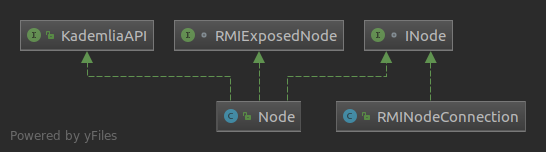
\includegraphics[width=0.7\textwidth]{images/Node.png}
    \end{center}
    \caption{Class hierarchy}   
\end{wrapfigure}

The RMINodeConnection class handles all the network communication and the possible exceptions/errors that come with it. The only difference within the node class between the two operating modes is that the class exposes itself via RMI providing the RMIExposedNode interface to the network when in network mode. Also the class uses its RMIExposedNode reference as its sender reference object for method calls on remote nodes. In local mode, the node uses the direct "this" reference as the sender for the method calls on remote nodes and does not expose itself via RMI. There is no other difference between the operating modes, as all the procedures always only refer to the general INode interface.

This is only operating mode specific code fragment in the Node class. It sets the reference that is used as the "sender" argument in the method calls on remote nodes and exposes the local node to the network if necessary:

\begin{minted}{java}
if(exposeRMI) {
    exposeRMI();
    //Use RMINodeConnection as sender (local address and port)
    localNode = new RMINodeConnection(address, port); 
}
else {
    //Use a direct reference as sender
    localNode = this;
}
\end{minted}

RMIExposedNode is the actual RMI that gets exposed and that is used within the RMINodeConnection class as the stub. The RMIExposedNode objects are wrapped in the RMINodeConnection class to make it compatible with the INode interface by handling network exceptions. The KademliaAPI interface is a simplified interface for the local user to control her node.

\subsection{Differences}

To implement Kademlia the specifications were followed as closely as possible. Anyhow there are still some differences between the specification and the implementation:

First of all Kademlia uses UDP for communication. This is the only specification about the communication protocol. For this implementation it was decided to use the TCP based Remote Method Invocation for communication. RMI is a very well tested way to communicate between remote Java applications. Reasons for this decision are the robustness of RMI and the fact that RMI is very well integrated into Java. Even though RMI uses TCP it does not hold connections for long. Because of this, RMI will not harm the performance of the network but it will make implementation easier and less error prone. Because of the encapsulation of the networking code, RMI can be easily replaced with a UDP module if needed in the future.

Because Kademlia needs to communicate with multiple nodes within the lookup procedure, this process can be sped up by running it in parallel. This will result in more hops but may decrease lookup time. In this work the goal was to keep the complexity of the implementation low and the benchmarks focused on the number of hops and did not record lookup time, as this would be very hard to simulate. Because of this, multi threading on lookup was not implemented. 

To avoid hot spots in Kademlia, caching is used in the original specification. This was not implemented in this version, as this feature was found to be not vital to Kademlia. As stated before, low complexity was prioritized over "bells and whistles".

In the specification of Kademlia the procedure of storing a value in the network is described as performing a node\_lookup and then storing the value in the closest k nodes. Thereby in the node\_lookup repeatedly the closest yet seen node will be asked for closer nodes and the procedure stops as soon as no closer node has been found. This results sometimes in the fact that values are stored quite far away from their closest node because a closer node could have been found by just asking a node that is slightly further away and holds a reference to that even closer node. 

To increase the chance that the values are actually stored as close as possible to the identifier, this implementation of Kademlia repeats the lookup until it does not find a closer node n times in a row; n is a configurable parameter. This way the mean number of hops of the setValue operation increases, but on the other hand the mean number of hops of the getValue operation decreased significantly.

\newpage
\section{Results}

This implementation of Kademlia was tested in two operation modes: With communication of the network and with communication within the process. The correctness of the implementation was tested using network communication and it can be concluded that it works. Because it is hard to test the implementation over the network with a large quantity of nodes, the benchmarks and churn tests were conducted in the second operation mode: Communication within the process.

\subsection{Churn tests}

Two churn tests were conducted. In the first experiment nodes were added to and removed from the network repeatedly. In 100 repetitions each time a random amount of nodes, up to half of all nodes in the network, where removed. Then new nodes have been added to the network until it reached the initial number of nodes again.  After that initial churn one hundred values have been set at randomly chosen nodes and then looked up by other randomly chosen nodes to test the integrity of the network. It turns out that the network is stable and survived the initial churn.

In the second experiment a network has beed created and then repeatedly values have been set on n nodes, n - 1 nodes have been removed and the value was looked up. Even though lookup time increased in comparison to when the nodes are not removed, the network was able to always find the value. These two tests show that the network works quite well under churn.

\subsection{Performance tests}

To test the performance of the implementation a network of n nodes has been created. After the creation of the network, repeatedly values have been set at a randomly chosen node and looked up at another randomly chosen node. In this test 3000 values have been set and looked up. The number of hops for both setValue ("Store") and getValue ("Lookup") have been recorded as well as the number of known nodes for each node in the network ("State") at the end of the experiment.

% TODO: Vergleichswert aus der Literatur

\begin{figure}[ht]
    \caption{Store}
    \centering
    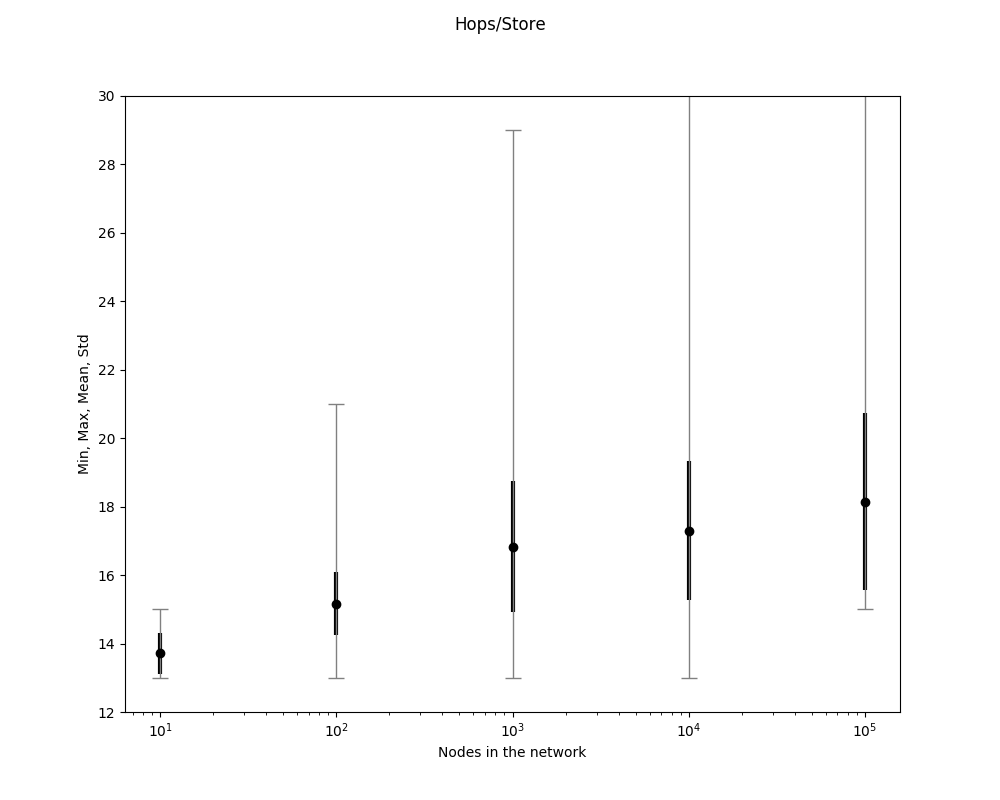
\includegraphics[width=0.80\textwidth]{images/set_figure.png}
\end{figure}

\begin{figure}[ht]
    \caption{Lookup}
    \centering
    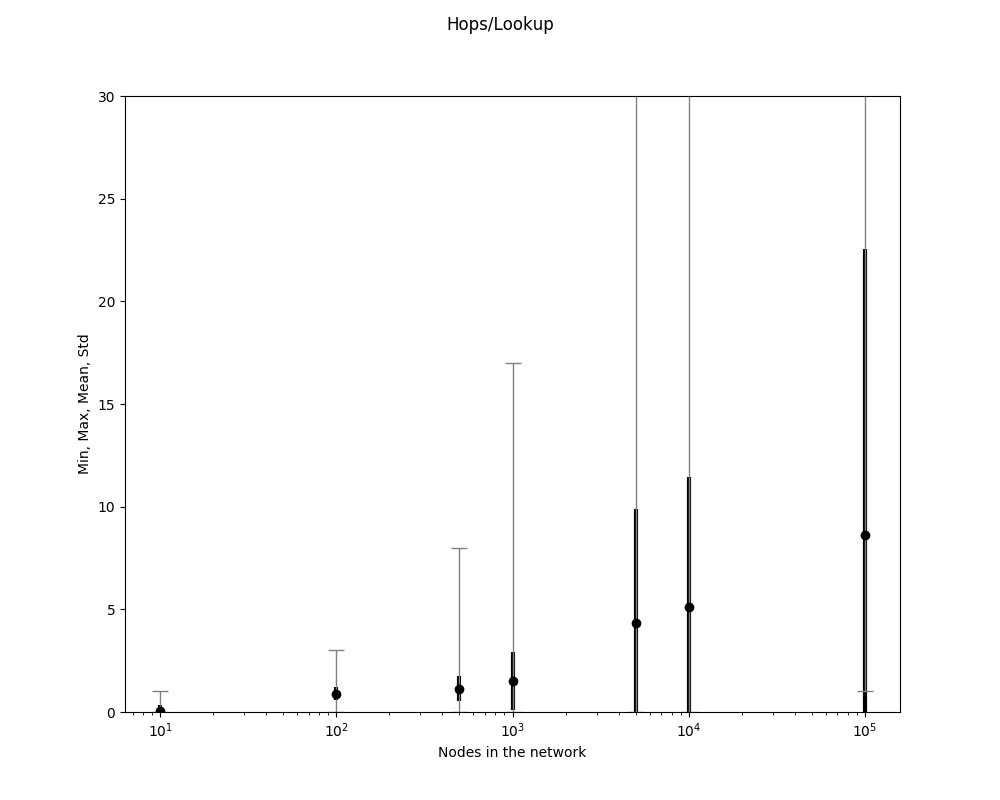
\includegraphics[width=0.80\textwidth]{images/lookup_figure.png}
\end{figure}

\begin{figure}[ht]
    \caption{State}
    \centering
    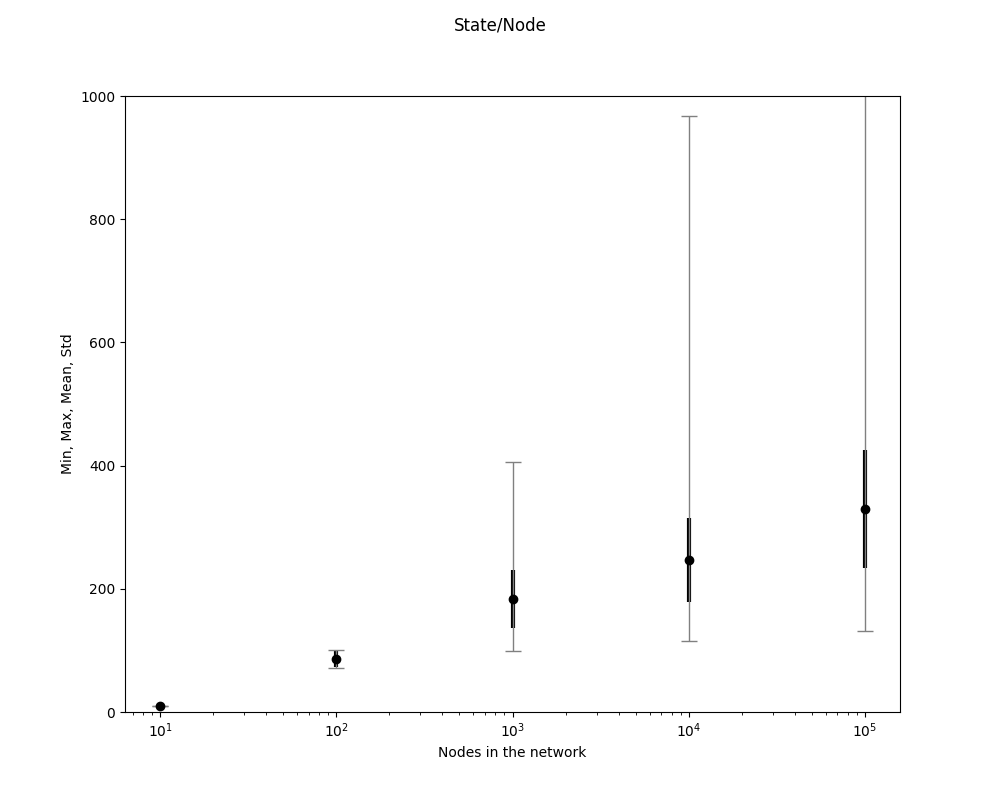
\includegraphics[width=0.80\textwidth]{images/state_figure.png}
\end{figure}

The X-axis represents the number of nodes in the network; note that the scale is logarithmic. The figures also contain information about the standard deviation and the min/max of the variables. As one can see, the complexity for the operations, as well as for the state of the network rise logarithmically to the number of nodes in the network. 

\clearpage

To evaluate the changed stopping condition of the node lookup, that was described earlier, performance tests were conducted with both the changed and the original stopping condition. Just to recap briefly: The original stopping condition for the node lookup stops the lookup as soon as no closer node is found. The changed stopping condition stops the lookup as soon as n times in a row no closer node is found. The parameter n was set to 5 in this test. 

\begin{table}[h]
\centering
\begin{tabular}{l*{6}{c}r}
Version           & Get mean & Get SD & Set mean & Set SD & State mean & State SD \\
\hline
Original          & 9        & 16     & 12       & 1      & 138        & 55       \\
Changed           & 4        & 5      & 17       & 2      & 223        & 61       \\
\end{tabular}
  \begin{tablenotes}
    \small
    \item Experiment with 5000 nodes
  \end{tablenotes}
\end{table}

The changed stopping condition resulted in more hops/set and more state/node but yielded a significantly lower mean of hops/get. It also reduced the standard deviation of the hops/get drastically. In this experiment a higher n lead to slower set operations and more state per node but also made the get operations much faster. In this implementation a fast get operation was the highest priority and therefore the changed stopping condition is used.

\newpage
\section{Conclusion}

% my experience / goals

The goal of the work was to learn about distributed hash tables by implementing one. Implementing a technology is a splendid way to learn it, as one needs to be aware of the "big picture" but also decide every detail of the implementation. In the end the learned material is documented unambiguously in code, as a nice side effect. Another advantage of this way of learning is, that it can be evaluated using very technical tools like performance and unit tests. This approach can be fully be recommended.

% benchmarks

The churn experiments show that this implementation of Kademlia maintains a robust network even under heavy churn. The experiments regarding the network performance show that this implementation reaches the expected efficiency of Kademlia. The store and lookup procedures operate with logarithmic time complexity in regard to the number of nodes in the network. Same goes for the growth of the state per node. 

% modifications

This implementation uses a different stopping condition for node lookup than the original specification. This modified stopping condition decreases the number of hops per lookup but increases the complexity of the store operation and grows the state on the nodes. As many networks perform far more lookups than store operations this might be a sensible modification to make in some situations. 

% outlook

This implementation of Kademlia misses the functionality of caching, hot-spot avoidance, parallel lookups and does use TCP instead of UDP. These features were not implemented as they were not regarded as vital to the Kademlia protocol. These would be good starting points for further development of the software.

% something about dhts in general?

\newpage
\section{References}
\printbibliography[heading=none]

\end{document}

% CITE
%Diese Arbeit \cite{Smith:2012qr} umfasst

% SECTION
%\section{Messung der Rechenzeit einzelner Zellen}
%\subsection{CustomShell}

% PICTURE
%\begin{figure}[ht]
%    \caption{Rechenzeiten visualisiert in XSimView}
%    \centering
%    \includegraphics[width=0.8\textwidth]{messzeiten.png}
%\end{figure}

% MULTI PICTURE
%\begin{figure}[!tbp]
%  \centering
%  \begin{minipage}[b]{0.49\textwidth}
%    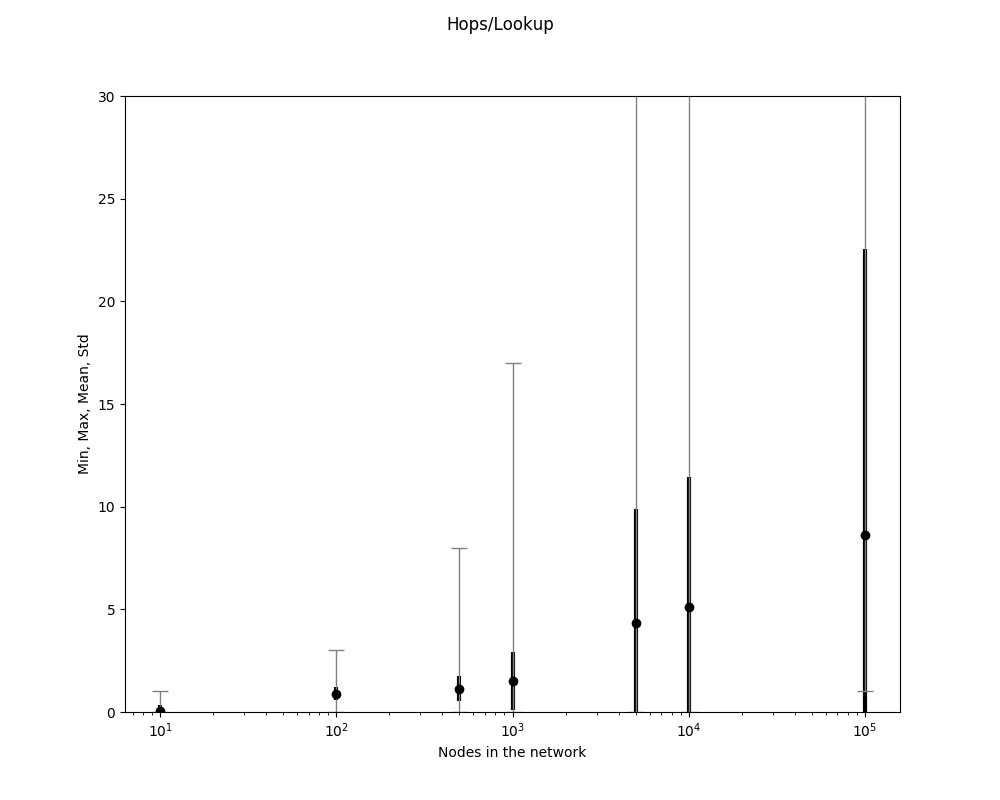
\includegraphics[width=\textwidth]{images/lookup_figure.png}
%    \caption{Lookup}
%  \end{minipage}
%  \hfill
%  \begin{minipage}[b]{0.49\textwidth}
%    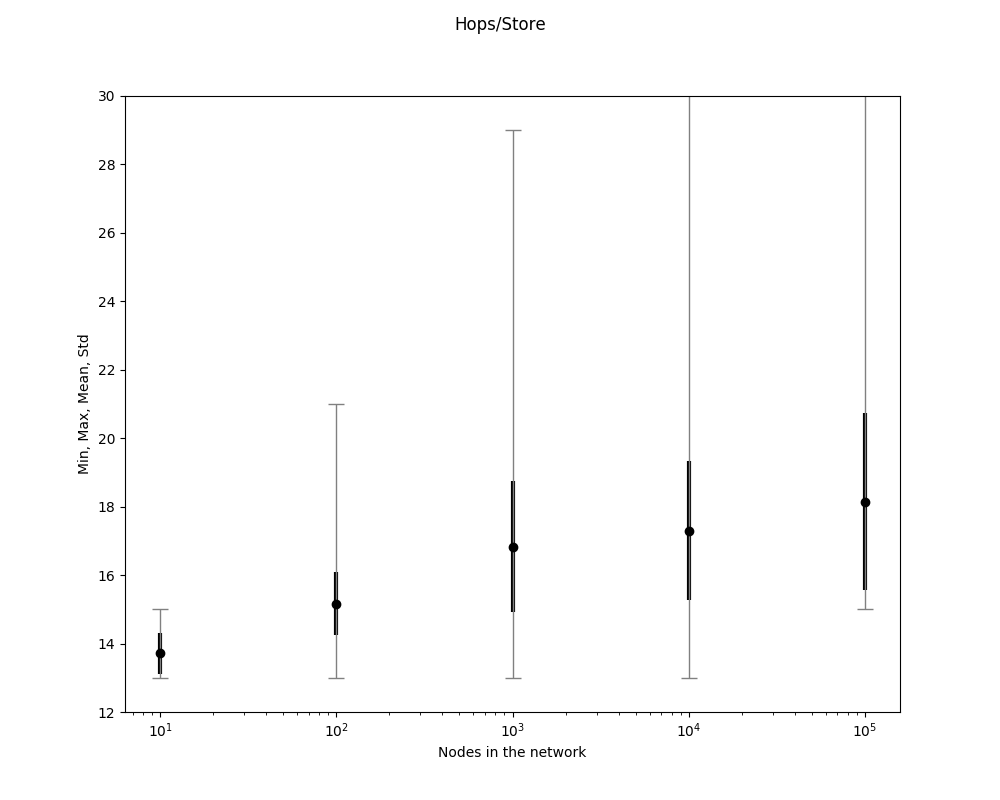
\includegraphics[width=\textwidth]{images/set_figure.png}
%    \caption{Store}
%  \end{minipage}
%\end{figure}

% TABLE
%\begin{tabular}{ l l }
%    outfiles.c & Filewriter f\"ur die Zeitmessung \\
%    fluxes.c & Durchf\"uhrung der Zeitmessung \\
%    cellinfo.h & Speicherung der Zeitmessung \\
%    globals.h & RecordCellCalculationTime Flag f\"ur Zeitmessung \\
%    interpreter.c & Erweiterungen des Interpreters \\
%    wrapper.c & Definition der NONE-Achse \\

% LIST
%\begin{enumerate}
%\item Stimulation of the SUT
%\item Observation of the reaction
%\item Comparison to the expected reaction
%\end{enumerate}

% CODE
%\begin{minted}{haskell}
%somecode
%\end{minted}

%The ideas of QuickCheck translate to Java very well. This is remarkable as QuickCheck originated %in functional programming and Java is inherently imperative. It was also shown that stateful code %can be tested elegantly and thoroughly with QuickCheck and Jqwik. 
%\end{tabular}
